\documentclass{standalone}
\usepackage{tikz}


\begin{document}

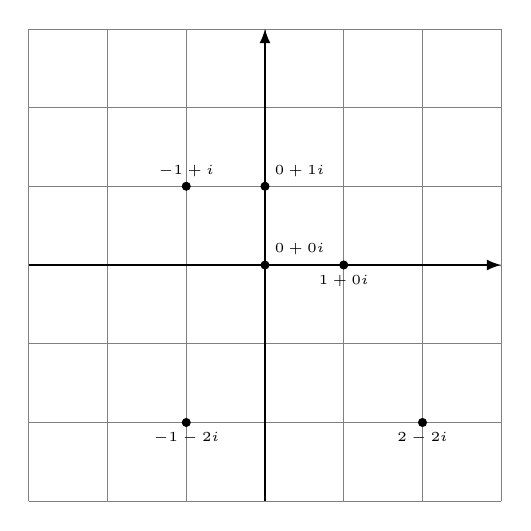
\begin{tikzpicture}
  \draw[help lines,black!50] (-3,-3) grid (3,3);
  \draw[thick,-latex] (-3,0) -- (3,0);
  \draw[thick,-latex] (0,-3) -- (0,3);

  \draw[fill=black] (0,0) circle [radius=0.05cm] node[anchor=south west,font=\tiny] {$0+0i$};
  \draw[fill=black] (0,1) circle [radius=0.05cm] node[anchor=south west,font=\tiny] {$0+1i$};
  \draw[fill=black] (1,0) circle [radius=0.05cm] node[anchor=north,font=\tiny] {$1+0i$};
  \draw[fill=black] (2,-2) circle [radius=0.05cm] node[anchor=north,font=\tiny] {$2-2i$};
  \draw[fill=black] (-1,-2) circle [radius=0.05cm] node[anchor=north,font=\tiny] {$-1-2i$};
  \draw[fill=black] (-1,1) circle [radius=0.05cm] node[anchor=south,font=\tiny] {$-1+i$};
\end{tikzpicture}

\end{document}